\section{Ambiente de desenvolvimento}

O trabalho prático e correspondente relatório foram desenvolvidos com recurso às tecnologias e ferramentas abaixo listadas:

\begin{itemize}
    \item Visual Studio Code 1.63.2;
    \item Node.js 17.3.0;
    \item Python 3.9.9;
    \item MongoDB 5.1.1;
    \item PostgreSQL 13;
    \item Mosquitto 2.0.13;
    \item Node-RED 2.1.4;
    \item GeoServer 2.19.4;
    \item PostGIS 3.1;
    \item Docker 20.10.11;
    \item Postman 9.8.2;
    \item Git 2.34.1;
    \item \LaTeX.
\end{itemize}

\clearpage

\section{Análise do problema}

O prelúdio do desenvolvimento do trabalho prático começou com a análise do problema a resolver. Para tal, procedeu-se à interpretação do respectivo enunciado, com vista a identificar os requisitos funcionais e não-funcionais da solução. Foram ainda definidos os devidos constrangimentos e pressupostos.

\subsection{Requisitos funcionais}

A tabela \ref{tab:rf} descreve os requisitos funcionais da solução.

\begin{table}[htb]
    \centering
    \resizebox{\textwidth}{!}{%
    \begin{tabular}{ll}
        \hline
        \textbf{Identificador} & \textbf{Descrição}                                                                         \\ \hline
        RF01                   & O sistema deverá suportar dois perfis de utilizador: gestores e clientes.                  \\
        RF02                   & O gestor deverá conseguir configurar diferentes tipologias de veículos.                    \\
        RF03                   & O gestor deverá ser capaz de definir o preçário para cada tipologia de veículo.            \\
        RF04                   & O gestor deverá conseguir gerir (adicionar, remover, etc.) a frota de veículos.            \\
        RF05                   & O gestor deverá ser capaz de consultar o estado e histórico de utilização do sistema.      \\
        RF06                   & Um novo cliente deverá conseguir registar-se no sistema.                                   \\
        RF07                   & A idade e género do cliente deverá ser inferido através do carregamento de uma fotografia. \\
        RF08                   & O cliente deverá ter a possibilidade de carregar o saldo associado ao seu perfil.          \\
        RF09                   & O cliente deverá conseguir consultar as tipologias de veículos e respectivos preçários.    \\
        RF10                   & O sistema deverá permitir que clientes encontrem o(s) veículo(s) mais próximo(s) de si.    \\
        RF11                   & O sistema deverá permitir o aluguer de veículos por clientes.                              \\
        RF12                   & O sistema deverá calcular o trajecto mais rápido entre a origem e o destino da viagem.     \\
        RF13                   & O custo de uma viagem deverá ser calculado com base no período de utilização.              \\
        RF14                   & O cliente deverá conseguir consultar as viagens efectuadas e respectivos detalhes.         \\
        RF15                   & O cliente deverá conseguir consultar o seu perfil e respectivos detalhes.                  \\ \hline
    \end{tabular}%
    }
    \caption{Requisitos funcionais da solução}
    \label{tab:rf}
\end{table}

\subsection{Requisitos não-funcionais}

A tabela \ref{tab:rnf} define os requisitos não-funcionais da solução.

\begin{table}[htb]
    \centering
    \resizebox{\textwidth}{!}{%
    \begin{tabular}{ll}
        \hline
        \textbf{Identificador} & \textbf{Descrição}                                                                           \\ \hline
        RNF01                  & O cliente deverá encontrar-se autenticado no sistema para que goze das suas funcionalidades. \\
        RNF02                  & O sistema deverá ser constituído por serviços com propósitos funcionais bem definidos.       \\
        RNF03                  & A API do sistema deverá estar documentada através da especificação Open API.                 \\
        RNF04                  & Deverá ser assegurada a resiliência, escalabilidade e disponibilidade do sistema.            \\
        RNF05                  & O sistema deverá ser disponibilizado através da orquestração de contentores.                 \\
        RNF06                  & Os contentores deverão ser concebidos com recurso a imagens oficiais.                        \\ \hline
    \end{tabular}%
    }
    \caption{Requisitos não-funcionais da solução}
    \label{tab:rnf}
\end{table}

\subsection{Constrangimentos e pressupostos}

A tabela \ref{tab:cp} identifica os constrangimentos e pressupostos da solução.

\begin{table}[htb]
    \centering
    \resizebox{\textwidth}{!}{%
        \begin{tabular}{ll}
        \hline
        \textbf{Identificador} & \textbf{Descrição}                                                                             \\ \hline
        CP01                   & Para realizar uma viagem, o cliente deverá dispor do saldo necessário.                         \\
        CP02                   & O cliente apenas poderá realizar viagens se tiver, pelo menos, 16 anos de idade.               \\
        CP03                   & Se o cliente ficar sem saldo no decorrer de uma viagem, o veículo deverá parar após um minuto. \\ \hline
        \end{tabular}%
    }
    \caption{Constrangimentos e pressupostos da solução}
    \label{tab:cp}
\end{table}

\section{Desenho da solução}

O desenho da solução envolveu fundamentalmente duas etapas: a elaboração da arquitectura do sistema e a arquitectura dos serviços. Esta secção discute ambas.

\subsection{Arquitectura do sistema}

A solução é baseada num sistema distribuído que segue uma arquitectura orientada a micro serviços. Neste, existe um conjunto de serviços vagamente acoplados, com propósitos funcionais bem definidos, que comunicam entre si, com vista a concretizar diferentes casos de uso. 

A figura \ref{fig:system-arch} ilustra um diagrama de componentes que especifica a arquitectura do sistema. Em seguida, é apresentada uma síntese de cada um dos componentes.

\begin{figure}[htb]
    \centering
    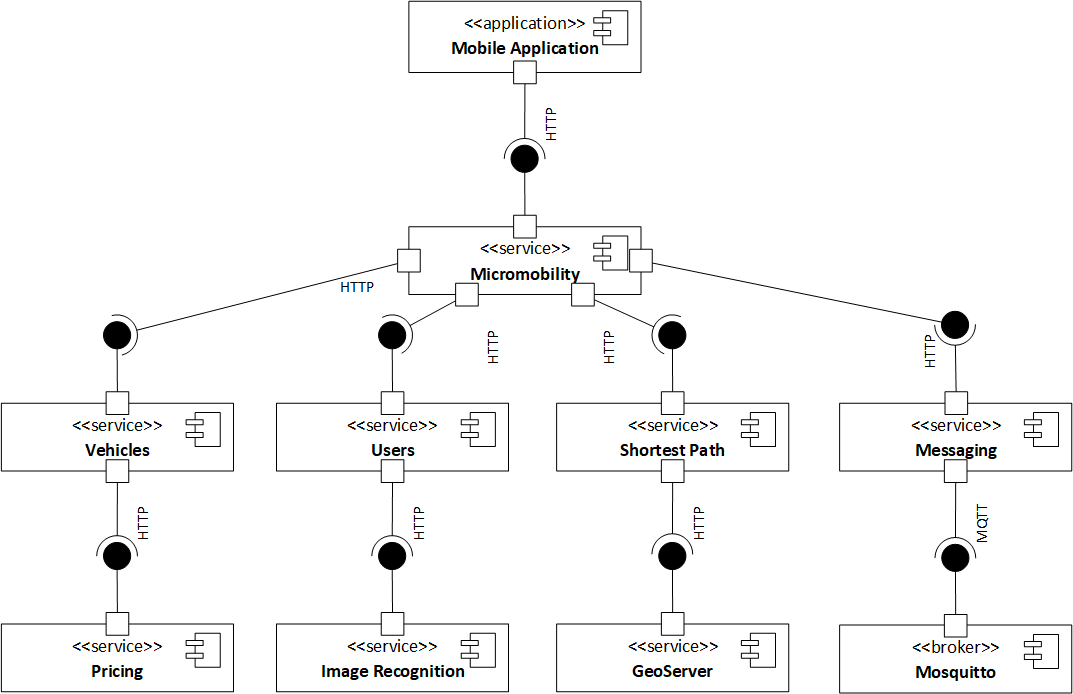
\includegraphics[width=1\textwidth]{img/system-arch.png}
    \caption{Arquitectura do sistema}
    \label{fig:system-arch}
\end{figure}

\subsubsection{Pricing}

Serviço orientado à gestão e armazenamento de tipologias de veículos e preçários. É independente na medida em que não depende de nenhum outro serviço.

\subsubsection{Image Recognition}

Como o nome sugere, trata-se de um serviço focado no reconhecimento de imagem. Através deste, com recurso a inteligência artificial, é possível estimar a idade e género de um determinado indivíduo. Não apresenta nenhuma dependência. 

\subsubsection{GeoServer}

Serviço de código aberto cujo propósito é a partilha, processamento e edição de dados geoespaciais. Suporta múltiplos formatos de dados.

\subsubsection{Mosquitto}

Serviço de código aberto responsável por mediar mensagens entre processos através do protocolo MQTT. Considerando a sua natureza leve, possibilita uma integração eficiente dos serviços do sistema com os veículos associados.

\subsubsection{Vehicles}

Serviço que está a cargo de gerir e armazenar os veículos. Depende de consultas ao serviço de gestão e armazenamento de tipologias de veículos e preçários.

\subsubsection{Users}

Serviço capaz de gerir e armazenar os utilizadores, independentemente de estes serem gestores ou clientes. Depende do serviço de reconhecimento de imagem para, no momento de registo de um cliente, estimar o seu género e validar a sua idade.

\subsubsection{Shortest Path}

Serviço que se apresenta como uma abstracção ao serviço de processamento de dados geoespaciais. Permite, essencialmente, calcular o caminho mais curto entre dois pontos geográficos.

\subsubsection{Messaging}

Serviço cujo intuito é interpretar as mensagens provenientes dos veículos e desencadear as operações adequadas nos serviços. Para tal, subscreve os  tópicos existentes no serviço capaz de mediar eventos, previamente descrito.

\subsubsection{Micromobility}

Serviço incumbido de definir as operações de alto nível do sistema. Concretiza o comportamento funcional do sistema por meio da orquestração dos restantes serviços. Em termos conceptuais, este serviço assume o papel de gateway, isolando clientes (e, por consequência, utilizadores) dos restantes serviços.

\subsubsection{Mobile Application}

Aplicação móvel com a qual o utilizador interage para satisfazer os casos de uso previstos na etapa de análise do problema. Esta comunica exclusivamente com o serviço de micromobilidade. O componente encontra-se fora do âmbito do projecto, pelo que é considerado trabalho futuro.

\subsection{Arquitectura dos serviços}

Os serviços do sistema seguem uma arquitectura de referência. Pretende-se, com esta decisão, promover a uniformidade, velocidade de desenvolvimento e facilidade de manutenção da solução. A única excepção é o serviço de reconhecimento de imagem, dadas as suas especificidades técnicas.

Internamente, a arquitectura de referência é composta por quatro camadas: rotas, controladores, modelos  e serviços.  Cada uma das camadas, assim como respectivos tipos, têm responsabilidades claramente definidas. Uma determinada camada apenas poderá invocar a camada que se encontra imediatamente abaixo.

Adicionalmente, considerando as boas práticas das arquitecturas orientadas a micro serviços, cada um dos serviços tem a sua própria base de dados.

A figura \ref{fig:service-arch} apresenta a arquitectura dos serviços. Depois, é exposta uma breve descrição de cada um dos seus componentes internos.

\begin{figure}[H]
    \centering
    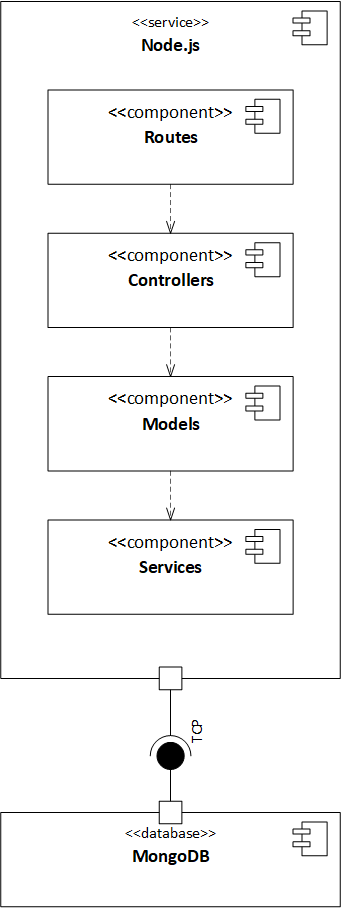
\includegraphics[width=0.3\textwidth]{img/service-arch.png}
    \caption{Arquitectura dos serviços}
    \label{fig:service-arch}
\end{figure}

\subsubsection{Routes}

Camada de apresentação do serviço. Expõe um conjunto de rotas responsáveis por concretizar as funcionalidades dispostas no serviço. A camada implementa um conjunto boas práticas características do domínio dos micro serviços:

\begin{itemize}
    \item Implementa a especificação REST e segue os princípios RESTful;
    
    \item Todas as rotas existentes encontram-se devidamente versionadas;
    
    \item Disponibiliza uma rota de monitorização que facilita eventuais automatismos inerentes à infraestrutura;
    
    \item Expõe um portal de documentação Swagger que descreve as rotas e modelos existentes no serviço;
    
    \item As respostas são enviadas no formato JSON. As mencionadas respostas são também comprimidas;
    
    \item Os pedidos, e respectivas respostas, estão sujeitas a um middleware dedicado a operações de logging;
    
    \item Emite, aquando das respostas, os códigos de estado HTTP adequados.
\end{itemize}

\subsubsection{Controllers}

Camada que define e reúne a lógica de negócio de alto nível do serviço. Seguindo um adequado isolamento e segmentação de responsabilidades, a camada que define as rotas, limita-se a invocar e a interpretar os resultados provenientes das rotinas presentes nesta camada. Por sua vez, esta camada invoca rotinas dispostas na camada imediatamente abaixo: a camada de modelos.

\subsubsection{Models}

Camada encarregue de definir e abstrair o modelo de dados utilizado na base de dados. Além disto, esta camada concentra os detalhes de execução das operações CRUD existentes no serviço, através de recursos definidos, configurados e expostos pela camada de mais baixo nível: a camada de serviços.

\subsubsection{Services}

Camada que estabelece a comunicação com a base de dados e restantes serviços do sistema. Esta camada faz uso extensivo de um ficheiro de configuração e define várias rotinas que definem eventos de logging que incentivam a uma adequada monitorização da infraestrutura.

\section{Disponibilização da solução}

A solução é disponibilizada através da conteinerização do sistema, onde cada um dos serviços até então descritos, assim como o motor de base de dados que sustenta os serviços, corresponde a um contentor específico.

A opção de decompor a solução em diversos contentores, fundamenta-se no facto de esta decomposição permitir escalar individualmente cada um dos serviços, consoante necessidades particulares. Consequentemente, de um ponto de vista de infraestrutura, esta decisão sustenta adequadamente a escalabilidade e disponibilidade da solução, sobretudo quando aliada a sistemas de orquestração.

Adicionalmente, com vista a promover a resiliência da solução, os contentores do sistema estão configurados para serem automaticamente reiniciados, em caso de falha não tratada.

\section{Resultados}

\subsection{Objectivos alcançados}

Considerando os requisitos funcionais, requisitos não-funcionais, constrangimentos e pressupostos oriundos da etapa de análise do problema, assim como os artefactos resultantes da etapa de desenho e desenvolvimento da solução, conclui-se que a basta maioria dos objectivos foram alcançados e que o sistema satisfaz os casos de uso inicialmente propostos.

Não obstante, tratando-se de uma primeira versão do sistema, existe espaço para melhorias. Estas melhorias consistem, fundamentalmente, no refinamento de pormenores não-funcionais, tais como o uso de um sistema de orquestração de contentores avançado (Kubernetes) ou a implementação de uma camada de autenticação e autorização em todos o serviços.

\subsection{Bonificações}

No decorrer da construção da solução, fez-se por implementar boas práticas de desenvolvimento de software, além das dispostas no enunciado do trabalho prático. Examine-se algumas das práticas empregues:

\begin{enumerate}
    \item O desenvolvimento da solução foi planeado e gerido através de metodologias de desenvolvimento ágeis, nomeadamente a framework Scrum, sendo que cada sprint teve a duração de uma semana, decorrida entre aulas dedicadas à unidade curricular;
    
    \item As operações de versionamento do sistema, recorrem ao sistema de controlo de versões git, cujo repositório encontra-se alojado na plataforma GitHub. Os elementos do grupo de trabalho têm o devido acesso ao repositório e podem, consequentemente, trabalhar em formato colaborativo;
    
    \item De modo a detectar erros e garantir a uniformidade do código fonte, fez-se uso de um linter, direccionado à linguagem de programação JavaScript, que se encontra convenientemente integrado nos serviços do sistema. O mesmo é apelidado de eslint e encontra-se ao abrigo de uma licença de código aberto;
    
    \item Com vista a promover a manutenção e simplicidade do código fonte, fez-se por seguir, na medida do possível, os princípios DRY e KISS.
\end{enumerate}

\subsection{Desafios de implementação}

O principal desafio de implementação da solução, foi o facto de alguns elementos do grupo de trabalho, terem pouco conhecimento ou experiência prévia na construção de sistemas distribuídos. Como expectável, este facto traduziu-se numa velocidade de implementação inicialmente reduzida, que foi progressivamente aumentando, à medida que o grupo de trabalho adquiria conhecimento, experiência e agilidade nas tecnologias e ferramentas utilizadas.